\chapter{\Large Introduction}
\label{introchap}

%%%%%%%%%%%%%%%%%%%%%%%%%%%%%%%%%%%%%%%%%%%%
%%%%%%%%%%%%%%%%%%%%%%%%%%%%%%%%%%%%%%%%%%%%
%%%%%%%%%%%%%%%%%%%%%%%%%%%%%%%%%%%%%%%%%%%%
%%%%%%%%%%%%%%%%%%%%%%%%%%%%%%%%%%%%%%%%%%%%
%						Introduction								%
%%%%%%%%%%%%%%%%%%%%%%%%%%%%%%%%%%%%%%%%%%%%
%%%%%%%%%%%%%%%%%%%%%%%%%%%%%%%%%%%%%%%%%%%%
%%%%%%%%%%%%%%%%%%%%%%%%%%%%%%%%%%%%%%%%%%%%
%%%%%%%%%%%%%%%%%%%%%%%%%%%%%%%%%%%%%%%%%%%%

Large scale systems consisting of many interacting subsystems are increasingly common, with examples such as computer networks, smart grids, and robotic sensor networks. The objectives for these applications are often complex; even centralized methods must make tradeoffs between performance and speed in order to optimize these non-convex, nonlinear systems. However, due to inherent limitations in computation, communication, or sensing, large multi-agent systems are often controlled in a distributed fashion. Here, individual agents, or subsystems, must make decisions based on local, often incomplete information, potentially exacerbating tradeoffs between performance and speed. Furthermore, the distributed nature of these multi-agent systems may introduce vulnerabilities to adversarial manipulation: by influencing small subsets of agents, a malicious agent may be able to degrade a system's overall performance.
The overarching goals of this dissertation are to (1) characterize tradeoffs between speed, performance, vulnerability, and information available to agents in distributed control systems, and (2) design algorithms with desirable guarantees in these aspects. 
In order to address these goals, we focus specifically on the following questions:


%%%%%%%%%%%%%%%%%%%%%%%%%%%%%%%%%%%%%%%%%%%%
%%%%%%%%%%%%%%%%%%%%%%%%%%%%%%%%%%%%%%%%%%%%
%%%%%%%%%%%%%%%%%%%%%%%%%%%%%%%%%%%%%%%%%%%%
%%%%%%%%%%%%%%%%%%%%%%%%%%%%%%%%%%%%%%%%%%%%
%						Research Questions							%
%%%%%%%%%%%%%%%%%%%%%%%%%%%%%%%%%%%%%%%%%%%%
%%%%%%%%%%%%%%%%%%%%%%%%%%%%%%%%%%%%%%%%%%%%
%%%%%%%%%%%%%%%%%%%%%%%%%%%%%%%%%%%%%%%%%%%%
%%%%%%%%%%%%%%%%%%%%%%%%%%%%%%%%%%%%%%%%%%%%

\begin{itemize}[leftmargin=*]
\item \textbf{When is fast convergence to near-optimal behavior possible in a distributed system?} (Chapter~\ref{ch2})
\item\textbf{Can agents in a distributed system learn near-optimal correlated behavior despite severely limited information about one another's behavior?} (Chapter~\ref{ch3})
\item\textbf{How does the structure of agent interaction impact the system's vulnerability to adversarial manipulation?} (Chapter~\ref{ch4})
\end{itemize}

This dissertation focuses on game theoretic methods of distributed control, which provide a framework for prescribing agents' control laws in a distributed control system \cite{Marden2008, Zhu2009, Goto2010, Staudigl2012, Fox2010, Lasaulce2011, Alpcan2010, Han2012, MacKenzie2006, Menache2011}. We begin by providing an informal background on game theoretic distributed control, and then we informally state the contributions of this thesis, as prompted by the three research questions above. This informal discussion will be followed by a formal development of necessary background materials, and then a formal summary of  contributions. 

%%%%%%%%%%%%%%%%%%%%%%%%%%%%%%%%%%%%%%%%%%%%
%%%%%%%%%%%%%%%%%%%%%%%%%%%%%%%%%%%%%%%%%%%%
%%%%%%%%%%%%%%%%%%%%%%%%%%%%%%%%%%%%%%%%%%%%
%%%%%%%%%%%%%%%%%%%%%%%%%%%%%%%%%%%%%%%%%%%%
%						Informal GT background    						%
%%%%%%%%%%%%%%%%%%%%%%%%%%%%%%%%%%%%%%%%%%%%
%%%%%%%%%%%%%%%%%%%%%%%%%%%%%%%%%%%%%%%%%%%%
%%%%%%%%%%%%%%%%%%%%%%%%%%%%%%%%%%%%%%%%%%%%
%%%%%%%%%%%%%%%%%%%%%%%%%%%%%%%%%%%%%%%%%%%%

\section{Background: Game theoretic distributed control}

Agents' control laws are a crucial component of any multi-agent system. They dictate how individual agents process locally available information to make decisions. Factors that determine the quality of a control law include informational dependencies, asymptotic performance guarantees, convergence rates, and resilience to adversarial influence.

In a game theoretic control law, each agent is assigned a {\it utility function}\footnote{The terms ``utility" and ``payoff" will refer to individual agents' utility functions, whereas ``objective" or ``welfare" will refer to the system level objective function. Note that in the social sciences literature, ``welfare" often refers to the sum of agents' utilities; in this dissertation the term will be used more broadly. By design, maximization of the global objective function will often coincide with maximization of the sum of agents' utilities. } and a {\it learning rule}.\footnote{The terms ``learning rule," ``revision strategy," and ``decision making strategy" will all refer to individual agents' learning rules.} Significant research has been directed at deriving distributed utility functions and learning rules that enable agents to make decisions based on limited information and also have desirable performance guarantees.


\noindent{\it \emph{Utility functions: what should agents optimize?} } 

An agent's local utility function dictates {\it what} it should seek to optimize. Well-studied utility functions from the literature include {\it marginal contribution} \cite{Wolpert1999}, {\it equal share} \cite{Arslan2007, Marden2008}, and {\it Shapley value} \cite{Shapley1964} utilities. Effective utility functions such as these are typically aligned with the global objective function. This means that when the system is near a globally optimal configuration, individual agents are also performing well with respect to their local utility functions.  An agent's individual utility function may depend on its own action and on available information about other agents' actions. This interdependence is desirable because an agent's best action with respect to the global objective often depends on the behavior of others. For example, if a subset of agents fails, the remaining agents should compensate accordingly; interdependent utility functions can enable this.

However, interdependence in agents' utility functions adds complexity to the distributed optimization problem. Individual agents do not have full control over the functions they seek to optimize. This can often lead to the existence of undesirable equilibria. Example~\ref{e:interdependent utilities} demonstrates a simple situation where undesirable equilibria can emerge if agents simply choose the optimal action, conditioned on others' actions.
The existence of inefficient equilibria motivates the study of alternative decision making rules which can act as methods for selecting desired equilibria.

\begin{example}\label{e:interdependent utilities}
Suppose we have two agents, {\it agent 1} and {\it agent 2}. Each agent can attempt to perform one of two tasks, {\it task 1}, which has a value of 10 if completed, or {\it task 2}, which has a value of 1 if completed.  The two agents can observe each other's behavior, but cannot communicate to coordinate their actions. Suppose that the agents can accomplish either task by working together on it, but they cannot accomplish either if they miscoordinate. This scenario is depicted in Figure~\ref{t:simple coordination}.

Because the agents can observe each other's actions, they have sufficient information to evaluate the global objective function. Hence we can simply assign agents' utilities to equal the global objective.\footnote{Assigning utilities equal to the global welfare is often impossible when agents do not have access to global information about others' actions.} Even in this simple situation, where agents have global knowledge of the system objective function and their utilities are exactly equal, {\it inefficient Nash equilibria} can emerge.

Informally, in a Nash equilibrium, no agent can improve its utility via a unilateral change of action. In this example, there are two Nash equilibria: an {\it efficient}, or welfare maximizing, equilibrium when the two agents coordinate on task 1, and another {\it inefficient}, or suboptimal, equilibrium when the two agents coordinate on task 2. When agents simply optimize their utilities conditioned on others' behavior, they may settle on either an inefficient or an efficient equilibrium. Furthermore, the performance loss associated with inefficient equilibria is not necessarily bounded. In this example, the difference in value between task 1 and task 2 could be very large, but collaboration on the less valuable task would remain a Nash equilibrium and a possible rest point of a simple utility maximization decision making strategy.



\begin{figure}
\begin{center}
\begin{tabular}{rr|c|c|}
\multicolumn{1}{c}{}&\multicolumn{3}{c}{\textbf{\underline{System objective}}}\\
\multicolumn{2}{r}{}&\multicolumn{2}{c}{\textbf{agent 2}}\\
\multicolumn{2}{r}{}
 &  \multicolumn{1}{c}{task 1}
 & \multicolumn{1}{c}{task 2} \\
\cline{3-4}
\multirow{2}{*}{\textbf{agent 1}}
&task 1 & 10 & 0 \\
\cline{3-4}
&task 2 & 0 & 1 \\
\cline{3-4}
\end{tabular}\quad\quad\quad
\begin{tabular}{rr|c|c|}
\multicolumn{1}{c}{}&\multicolumn{3}{c}{\textbf{\underline{Agent utilities}}}\\
\multicolumn{2}{r}{}&\multicolumn{2}{c}{\textbf{agent 2}}\\
\multicolumn{2}{r}{}
 &  \multicolumn{1}{c}{task 1}
 & \multicolumn{1}{c}{task 2} \\
\cline{3-4}
\multirow{2}{*}{\textbf{agent 1}}
&task 1 & \cellcolor[gray]{0.8}10,10 & 0,0 \\
\cline{3-4}
&task 2 & 0,0 & \cellcolor[gray]{0.8}1,1 \\
\cline{3-4}
\end{tabular}
\end{center}
\caption{A simple coordination task, with the system objective function on the left, and a possible choice of agent utilities on the right. Here, the goal is to design agents' utilities so that they coordinate to accomplish a task. Task 1 is more important than task 2. The shaded boxes represent Nash equilibria: neither agent can improve its utility via a unilateral change of action. Coordination on task 2 does not maximize the overall objective or agents' utilities, and is known as an {\it inefficient Nash equilibrium.} One objective in designing effective agent learning rules is to select a Nash equilibrium which also maximizes the objective, namely coordination on task 1.}
\label{t:simple coordination}
\end{figure}

\FloatBarrier
\end{example}



\noindent{\it \emph{Learning rules: how should agents optimize?}} 

An agent's learning rule dictates {\it how} it should optimize its utility function. In some cases, it may suffice for each agent to choose the action which maximizes its utility function, given others' current behavior. This is know as a {\it best response} learning rule. However, in many distributed systems, this approach can lead to undesirable equilibria, as shown in Example~\ref{e:interdependent utilities}. Alternative learning rules, such as log-linear learning \cite{Blume1993}, regret matching \cite{Foster2006, Marden2007}, or fictitious play \cite{fp1,fp2}, have been studied in the literature. In particular, log-linear learning is a type of noisy best response learning rule which can lead agents toward a global objective optimizer in distributed control systems, provided agents' utilities are designed appropriately. Here, agents optimize their utilities most of the time, but occasionally make suboptimal choices. Log-linear learning and similar noisy best response rules will be the focus of this dissertation.

The combination of agents' utility functions and learning rules dictates system dynamics, and hence determines (1) performance with respect to the system level objective, and (2) speed of convergence. Furthermore, agents' abilities to evaluate their utility functions depends on locally available information. Thus, information available to agents also impacts system dynamics, and becomes a potential source for vulnerability.


%%%%%%%%%%%%%%%%%%%%%%%%%%%%%%%%%%%%%%%%%%%%
%%%%%%%%%%%%%%%%%%%%%%%%%%%%%%%%%%%%%%%%%%%%
%%%%%%%%%%%%%%%%%%%%%%%%%%%%%%%%%%%%%%%%%%%%
%%%%%%%%%%%%%%%%%%%%%%%%%%%%%%%%%%%%%%%%%%%%
%						Informal statement of contributions				%
%%%%%%%%%%%%%%%%%%%%%%%%%%%%%%%%%%%%%%%%%%%%
%%%%%%%%%%%%%%%%%%%%%%%%%%%%%%%%%%%%%%%%%%%%
%%%%%%%%%%%%%%%%%%%%%%%%%%%%%%%%%%%%%%%%%%%%
%%%%%%%%%%%%%%%%%%%%%%%%%%%%%%%%%%%%%%%%%%%%

\section{Informal statement of contributions}


Here, we informally summarize this dissertation's primary contributions in the area of game theoretic distributed control, with respect to the three research questions posed above.

\noindent{\it\emph{Research question \#1: When is fast convergence to near-optimal collective behavior possible in a distributed system? }}

\smallskip

\noindent \textbf{Contribution: Fast convergence to near-optimal collective behavior is possible when agents revise their actions according a a mild variant of log-linear learning, provided (1) agents' utilities are their marginal contribution to the system level objective, and (2) heterogeneity among agents is limited.}


One well-studied method of optimizing behavior in a multi-agent system is to assign agent utilities to be their {\it marginal contribution} to the overall system objective \cite{Wolpert1999}, and have agents make decisions according to the {\it log-linear learning} rule \cite{Blume1993}. In log-linear learning, agents primarily choose utility maximizing actions, but choose suboptimally with a small probability that decreases exponentially with respect to the associated payoff loss. In the long run, marginal contribution utilities with log-linear learning dynamics spends the majority of time at the global objective function maximizer. Unfortunately, worst-case convergence times for log-linear learning are known to be exponential in the number of agents, \cite{Shah2010} often rendering this game theoretic control method impractical for large-scale distributed systems. 

However, when system heterogeneity is limited, i.e., agents can be grouped into a small number of populations according to their action sets and impact on the objective function, a variant of log-linear learning achieves improved worst-case convergence times. In Chapter~\ref{ch2}, we build on the work of \cite{Shah2010} to derive this variant, which converges in near-linear time with respect to the number of agents. 

\noindent{\it \emph{Research question \#2: Can agents in a distributed system learn near-optimal correlated behavior despite severely limited information about one another's behavior? }}

\smallskip

\noindent\textbf{Contribution: Following the algorithm in Chapter~\ref{ch3}, agents with limited knowledge of each other's behavior can learn a utility-maximizing correlated equilibrium.}


Significant research has been directed at deriving distributed learning rules that possess desirable asymptotic performance guarantees and convergence rates and enable agents to make decisions based on limited information. The majority of this research has focused on attaining convergence to (pure) Nash equilibria under stringent information conditions \cite{Young2009, Frihauf2012, Foster2006, Boussaton2012, Poveda2013, Gharesifard2012}. Recently, the research focus has shifted to ensuring convergence to alternative types of equilibria that often yield more efficient behavior than Nash equilibria.  In particular, results have emerged that guarantee convergence to Pareto efficient Nash equilibria \cite{Marden2009,Pradelski2012}, potential function maximizers \cite{Blume1993, Marden2012}, welfare maximizing action profiles \cite{Marden2011, Arieli2012}, and the set of correlated equilibria \cite{Hart2000,Marden2013c,Aumann1987,Foster1997}, among others.  

In most cases highlighted above, the derived algorithms guarantee (probabilistic) convergence to the specified equilibria.  However, the class of correlated equilibria has posed significant challenges with regards to this goal. Learning algorithms that converge to an efficient correlated equilibrium are desirable because optimal system behavior can often be characterized by a correlated equilibrium. Unfortunately, the aforementioned learning algorithms, such as regret matching \cite{Hart2000}, merely converge to the {\it set} of correlated equilibria. This means that the long run behavior does not necessarily constitute a specific correlated equilibrium at any instance of time.


In Chapter~\ref{ch3} we design and analyze an algorithm that converges to a payoff maximizing coarse correlated equilibrium when agents have no direct knowledge of each others' behavior. Here, agents' utilities depend on collective behavior, but they have no way of evaluating the utility of alternative actions. Our algorithm uses a common random signal as a coordinating entity to eventually drive agents toward the desired collective behavior. In the long run, day to day behavior is selected probabilistically according to the payoff maximizing coarse correlated equilibrium.

 
\noindent{\it \emph{Research question \#3: How does the structure of agent interaction impact a distributed system's vulnerability to adversarial manipulation?}}

\smallskip

 \noindent\textbf{Contribution: If every subset of agent interacts with sufficiently many other agents, the system is more resilient to adversarial manipulation.}


Agents in a distributed system often interact and share information according to a network. The structure of this network not only has an impact on a distributed control algorithm's performance and speed, but also on its resilience to adversarial manipulation. A loosely connected network may be easier to influence, because an adversary could more easily manipulate the information available to subsets of agents, thereby creating impacts that cascade throughout the system. On the other hand, a well-connected network may be more difficult to influence in this way. In Chapter~\ref{ch4}, we investigate such vulnerabilities for  {\it graphical coordination games} \cite{Ullmann1977,Cooper1999} with agents revising their actions according to log-linear learning. Here, we provided a condition based on network structure which guarantees resilience in a graphical coordination game. 

%%%%%%%%%%%%%%%%%%%%%%%%%%%%%%%%%%%%%%%%%%%%
%%%%%%%%%%%%%%%%%%%%%%%%%%%%%%%%%%%%%%%%%%%%
%%%%%%%%%%%%%%%%%%%%%%%%%%%%%%%%%%%%%%%%%%%%
%%%%%%%%%%%%%%%%%%%%%%%%%%%%%%%%%%%%%%%%%%%%
%						Technical Preliminaries						%
%%%%%%%%%%%%%%%%%%%%%%%%%%%%%%%%%%%%%%%%%%%%
%%%%%%%%%%%%%%%%%%%%%%%%%%%%%%%%%%%%%%%%%%%%
%%%%%%%%%%%%%%%%%%%%%%%%%%%%%%%%%%%%%%%%%%%%
%%%%%%%%%%%%%%%%%%%%%%%%%%%%%%%%%%%%%%%%%%%%



\section{Technical Preliminaries}

In this section, we provide technical motivation for the study of game theoretic control algorithms, and we also establish the technical background and notation necessary to formally state the main contributions of this dissertation.

Consider a multi-agent system consisting of agents, $N = \{1,2,\ldots,n\}$, where each agent $i\in N$ has a finite action set, $A_i$. The set of joint actions will be denoted by $\mathcal{A} = \prod_{i\in N} A_i$,  and a joint action will be written as $$a = (a_1,a_2,\ldots,a_n)\in\mathcal{A},$$ or using the shorthand notation $$(a_i,a_{-i}) := (a_1,a_2,\ldots,a_i,\ldots,a_n)\in\mathcal{A}.$$ 


Suppose we aim to design agents' local control laws in order to maximize the global objective function, $W:\mathcal{A}\to \mathbb{R}.$ An agent's control law will be defined by a {\it utility function} and {\it learning rule}.


\subsection{Agent utility functions}


Each agent, $i\in N$, is assigned a utility function, $U_i: \mathcal{A}\to\mathbb{R},$ which maps each joint action to a value in $\R.$  When agents' information about others' actions is limited, utilities can be designed accordingly, e.g., taking the form $U_i:\prod_{j\in N_i\cup \{i\}}A_j\to \R,$ where $N_i$ represents the set of agent $i$'s neighbors, as defined by some underlying communication graph. Alternatively, agent utilities may incorporate additional information about an underlying system state, e.g., $U_i:\mathcal{A}\times X\to \R$, where $X$ represents a set of possible states of the surrounding environment.

A set of agents together with action sets and utility functions defines a game.

\begin{defn}
A {\it game} is a tuple $(N,\{A_i\}_{i\in N}, \{U_i\}_{i\in N})$ consisting of a set of agents, $N$, and their associated action sets, $\{A_i\}_{i\in N}$, and utility functions, $\{U_i\}_{i\in N}$.
\end{defn}

In the absence of any notion of dynamics over game, $G$, we often view the Nash equilibrium as a natural rest point, since it occurs when no agent can improve its utility by unilaterally changing its action, i.e., no agent has an incentive to unilaterally deviate from a Nash equilibrium.\footnote{Throughout this dissertation, a {\it Nash equilibrium} will refer to an action profile satisfying this definition, whereas an {\it equilibrium} will correspond to a rest point of some specified dynamics.}

\begin{defn}
For a game $G = \left(N,\{A_i\}_{i\in N},\{U_i\}_{i\in N}\right),$ action profile $a = (a_i,a_{-i})\in \mathcal{A}$ is a {\it Nash equilibrium} \cite{Nash1950} if it satisfies:
$$U_i(a)\geq U_i(a_i^\prime,a_{-i}),\quad \forall i\in N, a_i^\prime\in A_i$$
\end{defn}


Commonly studied utility functions include marginal contribution \cite{Wolpert1999}, equal share \cite{Arslan2007,Marden2008}, and Shapley value \cite{Shapley1964} utilities. In this dissertation, we focus primarily on marginal contribution utilities, as defined below.\footnote{Game theoretic utility design for distributed control systems is an emerging area \cite{Marden2013d}, and is not a topic of this thesis. We employ well-studied utility functions which are suitable for our distributed optimization purposes and focus our study on agents' learning rules and communication structure.} 



\begin{defn}
An agent's {\it marginal contribution}\cite{Wolpert1999} to the system objective, $W:\mathcal{A}\to \R$, corresponding to joint action $a = (a_i,a_{-i})\in \mathcal{A}$ is defined by:
$${\rm MC}_i(a) = W(a) - W(\emptyset,a_{-i}),$$
where $(\emptyset,a_{-i})$ represents removing agent $i$ from the system, while keeping other agents fixed at actions $a_{-i}\in \prod_{j\in N\setminus\{i\}}a_j.$
\end{defn}

Assigning agents' utilities to be their marginal contribution to the system welfare ensures that the optimal allocation corresponds to a Nash equilibrium. Furthermore, this choice of utility function defines a potential game.

\begin{defn}
A game $(N,\{A_i\}_{i\in N}, \{U_i\}_{i\in N})$ is a {\it potential game}\cite{Monderer1996} if there exists a potential function, $\phi:\mathcal{A}\to \R$ satisfying
$$\phi(a_i,a_{-i}) - \phi(a_i^\prime,a_{-i}) = U_i(a_i,a_{-i}) - U_i(a_i^\prime,a_{-i})$$
for all $i\in N,$ all $(a_i,a_{-i})\in \mathcal{A},$ and all $a_i^\prime\in A_i.$
\end{defn}

In fact, assigning agents' utilities to be their marginal contribution to the system objective defines a potential game with $\phi(a) = W(a),\,\forall a\in \mathcal{A},$ i.e., the potential function is equal to the system welfare function. This is useful, because there are well studied learning algorithms which converge to a potential function maximizer, e.g., log-linear learning \cite{Blume1993}, which we will discuss in detail in Section~\ref{s:learning rules}. 


Finally, marginal contribution utilities can also reduce informational requirements in certain classes of distribution control problems, as we show in  Example~\ref{e:resource allocation}.

\begin{example}\label{e:resource allocation}
Consider a resource allocation task, where we wish to allocate agents in $N = \{1,2,\ldots, n\}$ to a set of resources $R = \{r_1,r_2,\ldots,r_n\}$. Here, agent's action sets are a collection of subsets of $R$, i.e., $A_i\subseteq 2^R,$ so that an action $a_i\in A_i$ represents allocation of agent $i$ to subset $a_i\subseteq R.$

In resource allocation problems, the global welfare depends on the welfare attained at each resource. Typically, resource allocation problems have {\it separable welfare functions}:
\begin{equation}\label{e:separable welfare}W_{\rm global}(a) = \sum_{r\in R} W_r(\{a\}_r),\quad a\in\mathcal{A},\end{equation}
where $W_r:\mathcal{A}\to\R$ is the welfare function associated with resource $r\in R$, and $\{a\}_r$ represents the set of agents selecting resource $r$ in action profile $a$. 

It is straightforward to show that, when the global welfare function is separable, i.e., can be written as in \eqref{e:separable welfare}, an agent's marginal contribution is given by
$$MC_i(a_i,a_{-i}) = \sum_{r\in a_i}W_r\left(\{a\}_r\right) - W_r\left(\{a\}_r\setminus\{i\}\right).$$
Hence, agent $i$ only needs information about other agents allocated to resources $r\in a_i\subseteq R$ to evaluate its marginal contribution.
\end{example}


\subsection{Learning rules}\label{s:learning rules}

Agents' learning rules are the second component of a game theoretic control law. Learning rules dictate how agents process information in order to optimize their utility functions. Here, a game $G$ is repeated over time, producing a sequence of joint actions, $a(0), a(1),a(2),\ldots.$ At each time $t\in\N$, some subset of agents, $S\subseteq N$ has the opportunity to revise their actions independently according to a learning rule of the form:
$$a_i(t) = \Pi_i(\{a(\tau)\}_{\tau=0,1,\ldots,t-1};U_i(\cdot),$$
where $\Pi$ is a policy that may depend on the history of agents' joint actions, and on the form of agent $i$'s utility function. The precise form of a learning rule can vary, depending on the information available to agent $i$ at time $t$. For example, a learning rule may instead be based on a finite history of joint actions, or on estimated (rather than exact) information.

For concreteness, we now define two well studied learning rules: the {\it best response learning rule} and the {\it log-linear learning rule}.

\begin{defn}
Given a game $G = \left(N,\{A_i\}_{i\in N},\{U_i\}_{i\in N}\right)$, and an initial joint action $a(0)\in \mathcal{A},$ the {\it best response learning rule} proceeds by repeating the following steps at each time $t\in \N$:
\begin{enumerate}
    \item Select an agent $i\in N$ uniformly at random.\footnote{Although selecting an agent uniformly at random is a centralized task, it is possible to define a fully decentralized learning rule in which agents update their actions in continuous time according to arrival times associated with independent Poisson processes. In Chapter~\ref{ch2} we formally define such a learning rule, but here we restrict ourselves to discrete-time learning rules for simplicity.}
    \item Agent $i$ selects a ``best response" action, i.e., agent $i$ selects action
    $$a_i\in \argmax_{a_i^\prime\in A_i}U_i(a_i^\prime,a_{-i}),$$
    which maximizes its utility, given all other agents' current actions.
    \item The ensuing joint action at time $t+1$ is 
    $$a(t+1) = (a_i,a_{-i}(t)),$$ i.e., agent $i$ plays its best response action, and all other agents repeat their previous actions.
\end{enumerate}
\end{defn}

In potential games, the best response learning rule converges to a Nash equilibrium of the game. However, this Nash equilibrium need not be efficient. For example, recall the game defined in Example~\ref{e:interdependent utilities}, with the system welfare and agent utility functions below. Recall that, in this example, neither agent can accomplish a task alone; hence, if either agent is removed from the system the value of the system objective is zero.

%\begin{figure}
\begin{center}
\begin{tabular}{rr|c|c|}
\multicolumn{1}{c}{}&\multicolumn{3}{c}{\textbf{\underline{System objective}}}\\
\multicolumn{2}{r}{}&\multicolumn{2}{c}{\textbf{agent 2}}\\
\multicolumn{2}{r}{}
 &  \multicolumn{1}{c}{task 1}
 & \multicolumn{1}{c}{task 2} \\
\cline{3-4}
\multirow{2}{*}{\textbf{agent 1}}
&task 1 & 10 & 0 \\
\cline{3-4}
&task 2 & 0 & 1 \\
\cline{3-4}
\end{tabular}\quad\quad\quad
\begin{tabular}{rr|c|c|}
\multicolumn{1}{c}{}&\multicolumn{3}{c}{\textbf{\underline{Agent utilities}}}\\
\multicolumn{2}{r}{}&\multicolumn{2}{c}{\textbf{agent 2}}\\
\multicolumn{2}{r}{}
 &  \multicolumn{1}{c}{task 1}
 & \multicolumn{1}{c}{task 2} \\
\cline{3-4}
\multirow{2}{*}{\textbf{agent 1}}
&task 1 & \cellcolor[gray]{0.8}10,10 & 0,0 \\
\cline{3-4}
&task 2 & 0,0 & \cellcolor[gray]{0.8}1,1 \\
\cline{3-4}
\end{tabular}
\end{center}
%\end{figure}
\medskip

Indeed, this example is a potential game with agents' utilities defined by their marginal contribution to the system welfare, and potential function, $\phi,$ equal to the system objective, i.e.,
\begin{equation}
\phi(a) = 
\begin{cases}
10 & \text{if $a =$ (task 1,task 1)}\\
0 & \text{if $a =$ (task 1,task 2)}\\
0 & \text{if $a =$ (task 2,task 1)}\\
1 & \text{if $a = $ (task 2, task 2)}
\end{cases}
\end{equation}

Here, the best response process will converge to one of the two Nash equilibria shaded in grey, depending on the initial joint action, $a(0),$ and on the identity of the updating agent at each time. Hence, there is no guarantee that the best response process will select a welfare-optimizing Nash equilibrium.



Mathematically, the best response process defines a Markov chain over the joint action space. We provide mathematical background on Markov chains in Appendix~\ref{appendixA}. Transition probabilities for the Markov chain associated with the best response learning rule for the example above is shown in Figure~\ref{f:BR_MarkovChain}, and are also given by the probability transition matrix,
$$P = \begin{bmatrix}
1&0&0&0\\
0.5&0&0&0.5\\
0.5&0&0&0.5\\
0&0&0&1
\end{bmatrix}.$$
 This Markov chain has two stationary distributions.
$$\pi_1 = \begin{bmatrix} 1&0&0&0 \end{bmatrix},
\quad
\text{and}
\quad 
\pi_2 = \begin{bmatrix} 0&0&0&1\end{bmatrix},$$
where the four joint actions are in the order shown in Figure~\ref{f:BR_MarkovChain}.
With respect to the global objective function, $\pi_1$ is optimal, whereas $\pi_2$ is suboptimal. 

\begin{figure}
    \centering
    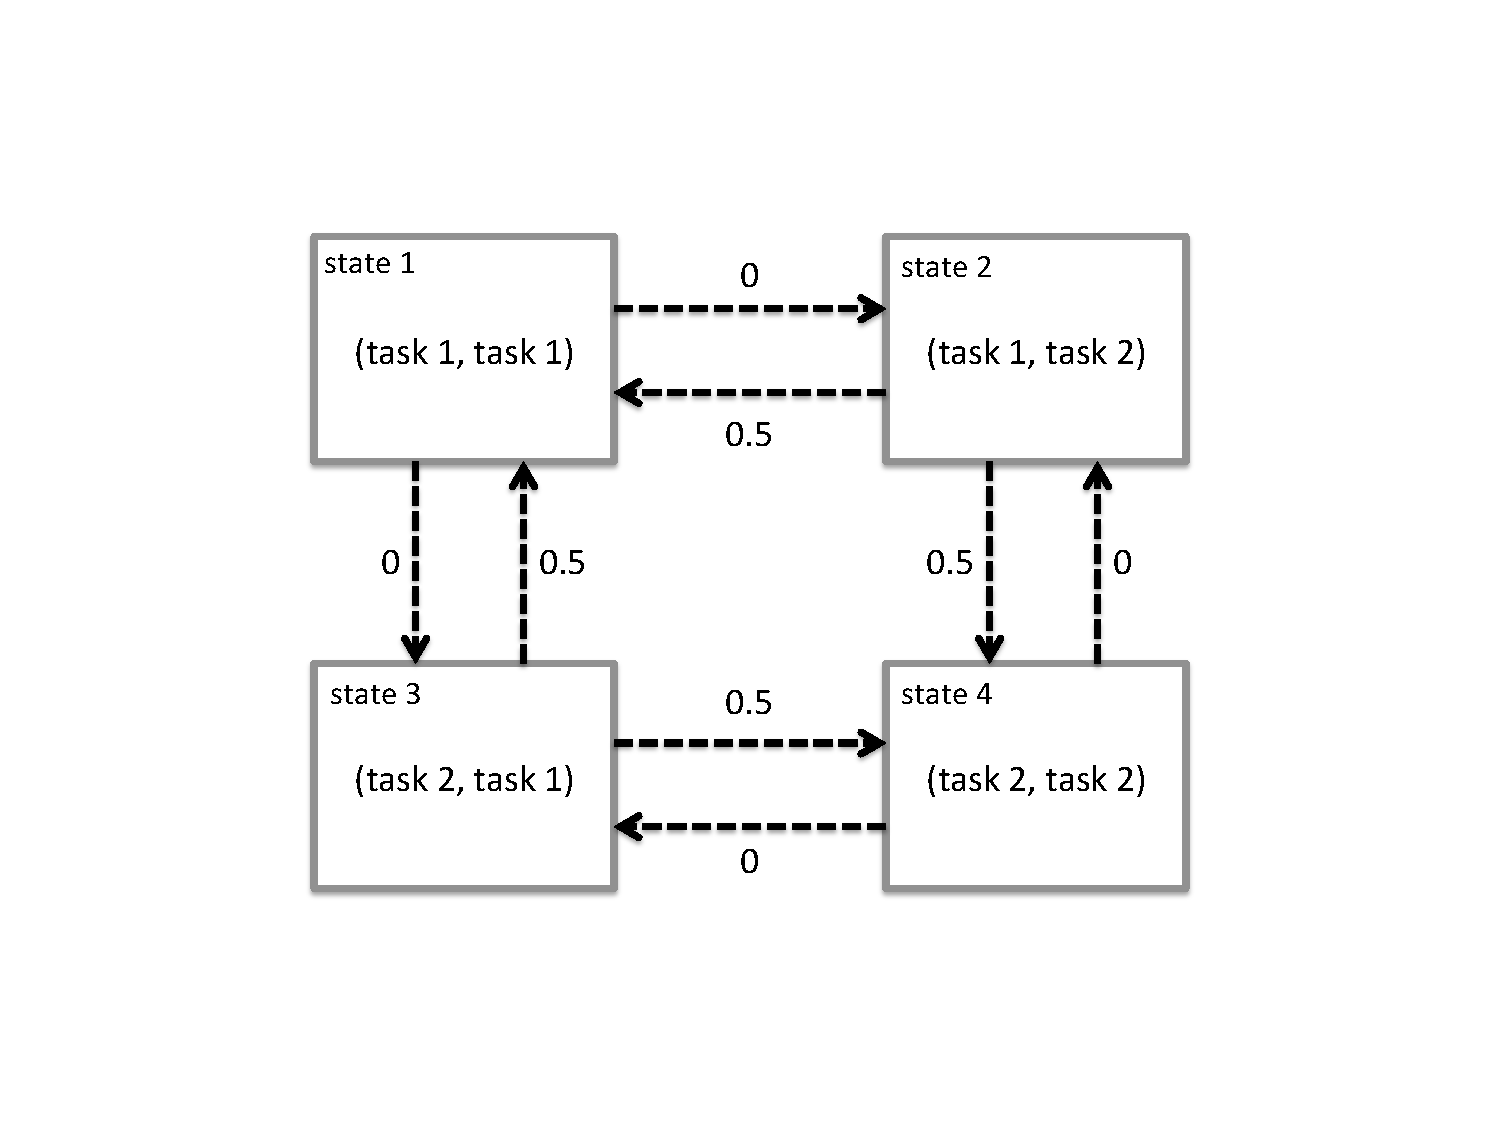
\includegraphics[scale=0.35, clip, trim=15mm 15mm 15mm 15mm]{BR_MarkovChain}
    \caption{Underlying Markov chain corresponding to the best response process over the game in Example~\ref{e:interdependent utilities}}
    \label{f:BR_MarkovChain}
\end{figure}

Log-linear learning belongs to the class of perturbed best response learning rules: here, an updating agent selects a best response action the majority of the time, but occasionally selects suboptimally. As we will show, log-linear learning acts as a method for selecting one of the (possibly many) stationary distributions of a best response process.

\begin{defn}
Given a game $G = \left(N,\{A_i\}_{i\in N}, \{U_i\}_{i\in N}\right)$, and an initial joint action $a(0)\in\mathcal{A},$ the {\it log-linear learning rule} proceeds by repeating the following steps at each time $t\in \N:$
\begin{enumerate}
    \item Select an agent $i\in N$ uniformly at random.
    \item Agent $i$ selects an action probabilistically, according to:
    \begin{equation}\label{e:LLL update}
        \Pr[a_i(t+1) = a_i] = {\exp\left(\beta U_i(a_i,a_{-i}(t)\right)\over
    \sum_{a_i^\prime\in A_i} \exp\left(\beta U_i(a_i^\prime,a_{-i}(t)\right)}
    \end{equation} 
    where $\beta$ is a design parameter.
    \item The ensuing joint action at time $t+1$ is $$a(t+1) = \left(a_i(t+1),a_{-i}(t)\right).$$
\end{enumerate}

\end{defn}

As parameter $\beta\to\infty$, an agent updating according to \eqref{e:LLL update} chooses a utility maximizing action with higher probability, and as $\beta\to 0,$ an updating agent chooses uniformly at random. The log-linear learning process defines a Markov chain over $\cal{A}$ with transition matrix $P^\beta$, parameterized by $\beta$. When the underlying game is a potential game with potential function $\phi$, the stationary distibution associated with the underlying Markov chain is given by 
\begin{equation}\label{e:LLL sd}
    \pi(a) = {\exp (\beta \phi(a))\over \sum_{a^\prime\in \cal{A}} \exp(\beta \phi(a)})
\end{equation}
From \eqref{e:LLL sd} it is straightforward to see that 
\begin{equation}
    \lim_{\beta\to\infty} \sum_{a\in \argmax \phi(a)} \pi_\beta(a) = 1.
\end{equation}
That is, as $\beta\to\infty$, log-linear learning converges to a stationary distribution, $\pi$, with full support on the potential maximizing actions. This limiting distribution is one of possibly many stationary distributions associated with the best response process. Hence, we often say that log-linear learning {\it selects} the desirable stationary distribution of the best response process. We refer to actions belonging to the support of this limiting distribution as {\it stochastically stable}, which we formally define in Appendix~\ref{appendixA}.



\begin{figure}
\vspace{.15in}
\begin{mdframed}
\underline{\textbf{Notation and Terminology}}
\begin{itemize}
    \item $N = \{1,2,\ldots,n\}$ - set of agents
    \item $A_i$ - agent $i$'s finite action set
    \item $\mathcal{A}:=\prod_{i\in N} A_i$ - the joint action space
    \item $a = (a_1,a_2,\ldots a_i,\ldots,a_n) = (a_i,a_{-i})\in\mathcal{A}$ - a joint action
    \item $W:\mathcal{A}\to\R$ - the system objective function. 
    \item $U_i:\mathcal{A}\to\R$ - agent $i$'s utility function
    \item ${\rm MC}_i(a)$ - agent $i$'s marginal contribution to the system objective at joint action $a\in \mathcal{A}$
    \item $\phi:\mathcal{A}\to \R$ - the potential function. Corresponds to the objective, $W$, when $U_i = {\rm MC}_i,\;\forall i\in N$.
\end{itemize}
\end{mdframed}
\end{figure}

\section{Formal summary of contributions}

In this section, we summarize the model associated with each of the three main contributions of this dissertation, and then formally state each contribution.\footnote{To ensure chapters are self-contained, we will repeat the formal model and definitions below in each.}

\noindent{\it\emph{Research question \#1: When is fast convergence to near-optimal collective behavior possible in a distributed system? }}


Here, we consider a game with agents $N = \{1,2,\ldots,n\}$. Each agent $i \in N$ has a finite action set denoted by $\aee_i$ and a utility function $U_i : \aee \rightarrow \mathbb{R}$, where $\aee = \prod_{i \in N} \aee_i$ denotes the set of joint actions.   We express an action profile $a \in \aee$ as $(a_i,a_{-i})$ where $a_{-i} = (a_1,\ldots,a_{i-1},a_{i+1},\ldots, a_n)$ denotes the actions of all agents other than agent $i$.  We denote a game $G$ by the tuple $G = \left(N, \{\aee_i\}_{i\in N}, \{U_i\}_{i \in N}\right)$\footnote{For brevity, we refer to $G$ by $G = \left(N, \{\aee_i\}, \{U_i\}\right)$. }.  



\begin{defn}\label{d:semi-anon potential}
%
A game $G$ is a semi-anonymous potential game if there exists a partition ${\cal N} = (N_1, N_2, \dots, N_m)$ of $N$ such that the following conditions are satisfied:

\smallskip

\noindent (i)  For any population $N_\l \in {\cal N}$ and agents $i,j \in N_\l$ we have $\aee_i = \aee_j$.  Accordingly, we say population $N_\l$ has action set $\bar{\aee}_\l= \{\a_\l^1,\a_\l^2,\ldots,\a_\l^{s_\l}\}$\footnote{We use the notation $\bar{\aee}_\ell$ to represent the action set of the $\ell$th population, whereas $\mathcal{A}_i$ represents the action set of the $i$th agent.} where $s_\l$ denotes the number of actions available to population $N_\l$.  For simplicity, let $p(i) \in \{1, \dots, m\}$ denote the index of the population associated with agent $i$.  Then, $\aee_i = \bar{\aee}_{p(i)}$ for all agents $i \in N$. 

\smallskip

\noindent(ii) For any population $N_\l \in {\cal N}$, let 
%
\begin{equation}
X_\l = \left\{\left({v_\l^1\over n},{v_\l^2\over n},\ldots,{v_\l^{s_\l}\over n}\right) \geq \mathbf{0} \st \sum_{k=1}^{s_\l} v_\l^k = |N_\l| \right\}
\end{equation}
%
represent all possible aggregate action assignments for the agents within population $N_\l$.  Here, the utility function of any agent $i \in N_\l$ can be expressed as a lower-dimensional function of the form $\bar{U}_i : \bar{\aee}_{p(i)} \times X \rightarrow \mathbb{R}$ where $X = X_{1} \times \dots \times X_m$.  More specifically, the utility associated with agent $i$ for an action profile $a = (a_i,a_{-i}) \in \aee$ is of the form $$U_i(a) = \bar{U}_i(a_i,a|_{X})$$ where
%
\begin{eqnarray}
a|_{X} &=& (a|_{X_1}, a|_{X_2},\ldots,a|_{X_m})\in X, \\
a|_{X_j} &=& \frac{1}{n}\left\{\left|\{j\in N_\l \st a_j = \a_\l^k\}\right|\right\}_{k=1,\ldots,s_\l}.
\end{eqnarray}
%
The operator $\cdot|_X$ captures each population's aggregate behavior in an action profile $\cdot$. 

\smallskip

\noindent(iii) There exists a potential function $\phi: X \to\R$ such that for any $a \in \aee$ and agent $i \in N$ with action $a_i' \in \aee_i$,
\small
\begin{equation}U_i(a) - U_i(a_i^{\prime},a_{-i}) = \phi(a|_X) - \phi((a_i^{\prime},a_{-i})|_X).\end{equation}
\normalsize
\end{defn}

Recall that assigning agents' utilities to be their marginal contribution to the system objective defines a potential game with $\phi(a) = W(a),\,\forall a\in \mathcal{A},$ i.e., the potential function is equal to the system objective function. Hence, we are often interested in studying algorithms which maximize the system potential. We now state Theorem~\ref{t:main theorem 1 ch2}, which is the main contribution of Chapter~\ref{ch2}.

\begin{restatable}{Theorem}{firsttheorem}\label{t:main theorem 1 ch2}
Let $G = (N,\{\mathcal{A}_i\},\{U_i\})$ be a semi-anonymous potential game with aggregate state space $X$ and potential function $\P:X\to [0,1].$ Suppose agents play according to a mild variant of log-linear learning, to be defined formally in Chapter~\ref{ch2}. Suppose further that the following conditions are met:         

\noindent (i)  The potential function is $\lambda$-Lipschitz, i.e., there exists $\lambda \geq 0$ such that
\begin{equation*}
|\P(x) - \P(y)|\leq\lambda\|x-y\|_1,\quad \forall x,y\in  X.
\end{equation*}

\noindent(ii) The number of players within each population is sufficiently large:
$$\sum_{i=1}^m |N_i|^2\geq \sum_{i=1}^m |\bar{\aee}_i| - m.$$  

\noindent For any fixed $\eps\in (0,1)$, if $\beta$ is sufficiently large, i.e., 
%
\begin{equation}\label{e:beta lb}
\beta\geq\max\left\{{4m(s-1)\over\eps}\log 2ms,{4m(s-1)\over\eps}\log{8ms \lambda\over\eps}\right\},
\end{equation}
%
then
%
\begin{equation}\label{e:expected val}
\E[\P(a(t)|_{X})]\geq\max_{x\in X}\P(x)-\eps
\end{equation}
%
for all
%
\small
\begin{align}
t&\geq \frac{2^{2ms}c_1 e^{3\beta}m(m(s-1))!^2 n}{4\alpha}\Biggl(\log\log (n+1)^{ms - m} +\log\beta+ 2\log{1\over\eps}\Biggr)\label{e:time requirement}
\end{align}
\normalsize
where $c_1$ is a constant that depends only on $s$.  
%
\end{restatable}

This theorem explicitly highlights the role of system heterogeneity, i.e., $m>1$ distinct populations, on convergence times of the process.  For the case when $m=1$, Theorem~\ref{t:main theorem 1 ch2} recovers the results of \cite{Shah2010}.  Observe that for a fixed number of populations, the convergence time grows as $n\log\log n$.  Furthermore, note that a small amount of system heterogeneity does not have a catastrophic impact on worst-case convergence times as suggested by Example~\ref{e:exIntro}.

\bigskip

\noindent{\it \emph{Research question \#2: Can agents in a distributed system learn near-optimal correlated behavior despite severely limited information about one another's behavior? }}

Here, we consider the framework of finite strategic form games where each agent $i \in N$ is associated with a finite action set $\aee_i$ and a utility function $U_i : \aee \rightarrow [0,1]$.
%For each agent $i\in N$, we extend the utility function $U_i$ to a function $U_i:\Delta(\mathcal{A})\to\R$ on the simplex over joint action space, $\Delta\mathcal{A}$, as follows:
%
%\begin{equation*}
%U_i(\q) = \sum_{a\in\mathcal{A}} U_i(a)q_a,\quad \quad \q = \{q_a\}_{a\in \mathcal{A}}\in \Delta(\mathcal{A}).
%\end{equation*}
%
We focus on the class of coarse correlated equilibria \cite{Aumann1987}.  A coarse correlated equilibrium is characterized by a joint distribution $q = \{q^a\}_{a \in \aee} \in \Delta(\aee)$, where $\Delta(\aee)$ represents the simplex over the finite set $\aee$, such that for any agent $i \in N$ and action $a_i' \in \aee_i$,
%
\begin{equation} 
\sum_{a \in \aee} U_i(a_i, a_{-i}) q^a \geq \sum_{a \in \aee} U_i(a_i', a_{-i}) q^a.
\end{equation}
%
We say a coarse correlated equilibrium $q^*$ is {\it efficient} if it maximizes the sum of the expected payoffs of the agents, i.e., 
%
\begin{equation}
%
q^* \in \underset{q \in {\rm CCE}}{\arg \max} \sum_{i \in N} \sum_{a \in \aee} U_i(a) q^a,
%
\end{equation}  
%
where ${\rm CCE} \subset \Delta(\aee)$ denotes the set of coarse correlated equilibria.  It is well known that ${\rm CCE} \neq \emptyset$ for any game $G$.

Note that the set of coarse correlated equilibria contains the set Nash equilibria; hence, the sum of agents' average payoff in an efficient correlated equilibrium is at least as large as the sum of agents' payoffs in an efficient Nash equilibrium.

We formally develop a learning algorithm in Chapter~\ref{ch3} which converges (in probability) to an efficient correlated equilibrium. Convergence to this equilibrium requires a degree of coupling in agents' utilities, which we refer to as interdependence.


\begin{defn}
A game $G$ with agents $N = \{1,2,\ldots,n\}$ is said to be {\it interdependent} if, for every $a\in\mathcal{A}$ and every proper subset of agents $J\subset N$, there exists an agent $i\notin J$ and a choice of actions $a_J^\prime\in\prod_{j\in J} \mathcal{A}_j$ such that $U_i(a_J^\prime,a_{-J})\neq U_i(a_J,a_{-J}).$
\end{defn}

Roughly speaking, the definition of interdependence states that it is not possibly to partition the group of agents into two sets whose actions do not impact one another's payoffs.

The following theorem characterizes the limiting behavior associated with the algorithm we will propose in Chapter~\ref{ch3}. 

\begin{restatable}{Theorem}{secondtheorem}\label{t:main theorem CCE}
%
Let $G = \left (N,\{U_i\},\{\mathcal{A}_i\}\right)$ be a finite interdependent game. 
%
First, suppose $q(S) \cap {\rm CCE} \neq \emptyset$.  Given any probability $p < 1$, if the exploration rate $\eps$ is sufficiently small, and if $\delta = \eps$, then for all sufficiently large times $t$, 
%
$$ {\rm Pr} \left[q(s(t)) \in \underset{ q \in q(S) \cap {\rm CCE}}{\arg \max} \ \sum_{i \in N} \sum_{a \in \aee} \ U_i(a) q^a \right] > p. $$ 
%
Alternatively, suppose $q(S) \cap {\rm CCE} = \emptyset$.  Given any probability $p < 1$, if the exploration rate $\eps$ is sufficiently small and $\delta = \eps$, then for all sufficiently large times $t$, 
%
$$ {\rm Pr} \left[q(s(t)) \in \underset{ q \in q(S)}{\arg \max} \ \sum_{i \in N} \sum_{a \in \aee} \ U_i(a) q^a \right] > p. $$ 
%
\end{restatable}

The condition $q(S) \cap {\rm CCE} \neq \emptyset$ implies the agents can realize specific joint distributions that are coarse correlated equilibria through the joint strategy set $S$.  When this is the case, the above algorithm ensures the agents predominantly play a strategy $s \in S$ where the resulting joint distribution $q(s)$ corresponds to the efficient coarse correlated equilibrium.  Alternately, the condition $q(S) \cap {\rm CCE} = \emptyset$ implies there are no agent strategies that can characterize a coarse correlated equilibrium.  When that is the case, the above algorithm  ensures the agents predominantly play strategies that have full support on the action profiles $a \in \aee$ that maximize the sum of the agents payoffs, i.e., $\arg \max_{a \in \aee} \sum_{i \in N} U_i(a)$.


\noindent{\it \emph{Research question \#3: How does the structure of agent interaction impact a distributed system's vulnerability to adversarial manipulation?}}

We use graphical coordination games, introduced in \cite{Cooper1999, Ullmann1977}, to study the impact of adversarial manipulation.  The foundation of a graphical coordination game is a simple two agent coordination game, where each agent must choose between one of two alternatives, $\{x,y\}$, with payoffs depicted by the following payoff matrix which we denote by $u(\cdot)$: 

\begin{center}
\begin{tabular}{r|c|c|}
\multicolumn{1}{r}{}	&\multicolumn{1}{c}{$x$}	&\multicolumn{1}{c}{$y$}\\
\cline{2-3}$x$			&$1+\alpha,\,1+\alpha$	&$0,\,0$\\
\cline{2-3}$y$			&$0,\,0$				&$1,\,1$\\
\cline{2-3}
\end{tabular}\\
\medskip
$2\times 2$ coordination game, $g$, with utilities $u(a_i,a_j),$ $a_i,a_j\in\{x,y\}$, and payoff gain $\alpha>0$
\end{center}
where $\alpha > 0$ defines the relative quality of conventions $(x,x)$ over $(y,y)$.  Both agents prefer to agree on a convention, i.e., $(x,x)$ or $(y,y)$, than disagree, i.e., $(x,y)$ or $(y,x)$, with a preference to agreeing on $(x,x)$.  
The goal of deriving local agent dynamics which lead to the efficient Nash equilibrium $(x,x)$ is challenging because of the existence of the inefficient Nash equilibrium $(y,y)$.  Deviating from $(y,y)$ for an individual agent is accompanied by an immediate payoff loss of $1$ to $0$; hence, myopic agents may be reluctant to deviate, stabilizing the inefficient equilibrium $(y,y)$.

This two player coordination game can be extended to an $n$-player {\it graphical coordination game}\cite{Kearns2001,Young2011, Montanari2010}, where the interactions between the agents $N=\{1, 2, \dots, n\}$ is described by an underlying graph $\mathcal{G} = (N,E)$ where $E \subseteq N\times N$ denotes the interdependence of agents' objectives.  More formally, an agent's total payoff is the sum of payoffs it receives in the two player games played with its neighbors ${\cal N}_i = \{j \in N : (i,j) \in E\}$, i.e., for a joint decision $a = (a_1, \dots, a_n) \in \{x,y\}^n$, the utility of agent $i$ is
%
\begin{equation}\label{e:original utility}
%
U_i(a_1, \dots, a_n) = \sum_{j \in {\cal N}_i} u(a_i, a_j).
%
\end{equation}

Log-linear learning \cite{Blume1993, Shah2010} is one distributed decision making rule that selects the efficient equilibrium, $\vec{x}$, in the graphical coordination game described above. Although agents predominantly maximize their utilities under log-linear learning, selection of the efficient equilibrium is achieved by allowing agents to choose suboptimally with some small probability that decreases exponentially with respect to the associated payoff loss. 

We study the potential for adversarial manipulation in the context of the above graphical coordination games. Here, we model the adversary as additional nodes/edges in our graph, where the action selected by these adversaries (which we fix as the inferior convention $y$) impacts the utility of the neighboring agents and thereby influences the agents' decision-making rule as specified by log-linear learning.  We focus on three different models of adversary behavior, referred to as {\it fixed, intelligent}; {\it mobile, random}; and {\it mobile, intelligent}.
%
\begin{itemize}
%
\item A fixed intelligent adversary aims to influence a fixed set $S\subseteq N$. To these agents the adversary appears to be a neighbor who always selects alternative  $y$.  We assume that $S$ is selected based on the graph structure ${\cal G}$ and $\alpha$.   
%
\item A mobile, random adversary connects to a random collection of agents $S(t)\subseteq N$ at each time, $t\in \mathbb{N}$ using no information on graph structure, $\mathcal{G},$ or payoff gain, $\alpha.$ 
%
\item A mobile, intelligent agent connects to a collection of agents, $S(t)\subseteq N$, at each time, $t\in \mathbb{N}$ using information on graph structure, $\mathcal{G}$, payoff gain $\alpha$, and the current action profile, $a(t)$.  
%
\end{itemize}
%
We formally define each of these three models for adversarial manipulation in Chapter~\ref{ch4}.

Consider the situation where agents in $N$ interact according to the graphical game $G$, and an adversary seeks to  convert as many agents in $N$ to play action $y$ as possible. 
At each time, $t\in \N$ the adversary attempts to influence a set of agents $S(t)\subseteq N$ by posing as a friendly agent who always plays action $y$. Agents' utilities, $\tilde{U}:\mathcal{A}\times 2^N\to\R$, are now a function of adversarial and friendly behavior, defined by:
\begin{equation}\label{e:new utility}
\tilde{U_i}((a_i,a_{-i}),S) = %U_i(a_i,a_{-i}) + \mathds{1}_{i\in S, a_i = y}
\begin{cases}
U_i(a_i,a_{-i})	&\text{if } i\notin S\\
U_i(a_i,a_{-i})	&\text{if } a_i = x\\
U_i(a_i,a_{-i}) + 1 &\text{if } i\in S,  a_i = y 
\end{cases}
\end{equation}
where $(a_i,a_{-i})\in\mathcal{A}$ represents friendly agents' joint action, and $S\subseteq N$ represents the set influenced by the adversary.
If  $i\in S(t)$, agent $i$ receives an additional payoff of 1 for coordinating with the adversary at action $y$ at time $t\in\N$; to agents in $S(t)$ the adversary appears to be a neighbor playing action $y$. By posing as a player in the game, the adversary has manipulated the utilities of agents belonging to $S$, providing an extra incentive to choose the inferior alternative, $y$. 

Suppose agents revise their actions according to log-linear learning, where the utility, $U_i$ defined in \eqref{e:original utility} is replaced by $\tilde{U}_i$ in \eqref{e:new utility}. 

A graphical coordination game $G$ is universally resilient to an adversary if $\vec{x}$ is strictly stochastically stable for all possible influenced sets $S(t)$, $t\in N$ and adversarial capability, $k\leq n.$ The following theorem provides sufficient conditions that ensure $G$ is universally resilient. For sets $S,T\subseteq N$, define
$$d(S,T) := |\{\{i,j\}\in E\st i\in S, j\in T\}|.$$

\begin{restatable}{Theorem}{thirdtheorem}\label{t:A stable all}
Let $\mathcal{G} = (N,E)$, and suppose an adversary influences some set $S(t)$ with $|S(t)| = k$ at each $t\in\N.$ If
\begin{equation}\label{e:YoungBound}
\alpha > {|T| - d(T,N\setminus T)\over d(T,N)},\quad\forall T\subseteq N
\end{equation}
Then $\vec{x}$ is strictly stochastically stable. In particular, if $|S(t)| = N$ for all $t\in \N$, \eqref{e:YoungBound} is also a necessary condition for strict stochastic stability of $\vec{x}$. 
\end{restatable}

Next, we analyze the case where agents are arranged according to a line. Values of $\alpha$ for which each type of agent can stabilize $\vec{y}$ in the line are summarized below and in Figure~\ref{f:barGraph}. Formal theorem statements associated with each are provided in Chapter~\ref{ch4}.
\begin{itemize}
\item A fixed, intelligent adversary with capability $k$ can stabilize joint action $\vec{y}$ when $\alpha<k\mathop{/}(n-1)$ (Theorem~\ref{t:fixed line graph}).
\item A mobile, random adversary with capability $k\leq n-1$ can stabilize joint action $\vec{y}$ when $\alpha <1$ (Theorem~\ref{t:mr ss}).
\item A mobile, intelligent adversary with capability $k=1$ can stabilize joint action $\vec{y}$ when $\alpha <1$ (Theorem~\ref{t:intelligent}).
\item A mobile, intelligent adversary with capability $k\geq 2$ can stabilize joint action $\vec{y}$ when $\alpha <n\mathop{/}(n-1)$ (Theorem~\ref{t:intelligent}).
\end{itemize}
Note that a mobile, random adversary's influence is the same for any capability $k$ with $1\leq k\leq n-1.$ Similarly, a mobile, intelligent adversary does not increase its influence on agents in a line by increasing its capability above $k=2.$

\begin{figure}[!]
  \centering
    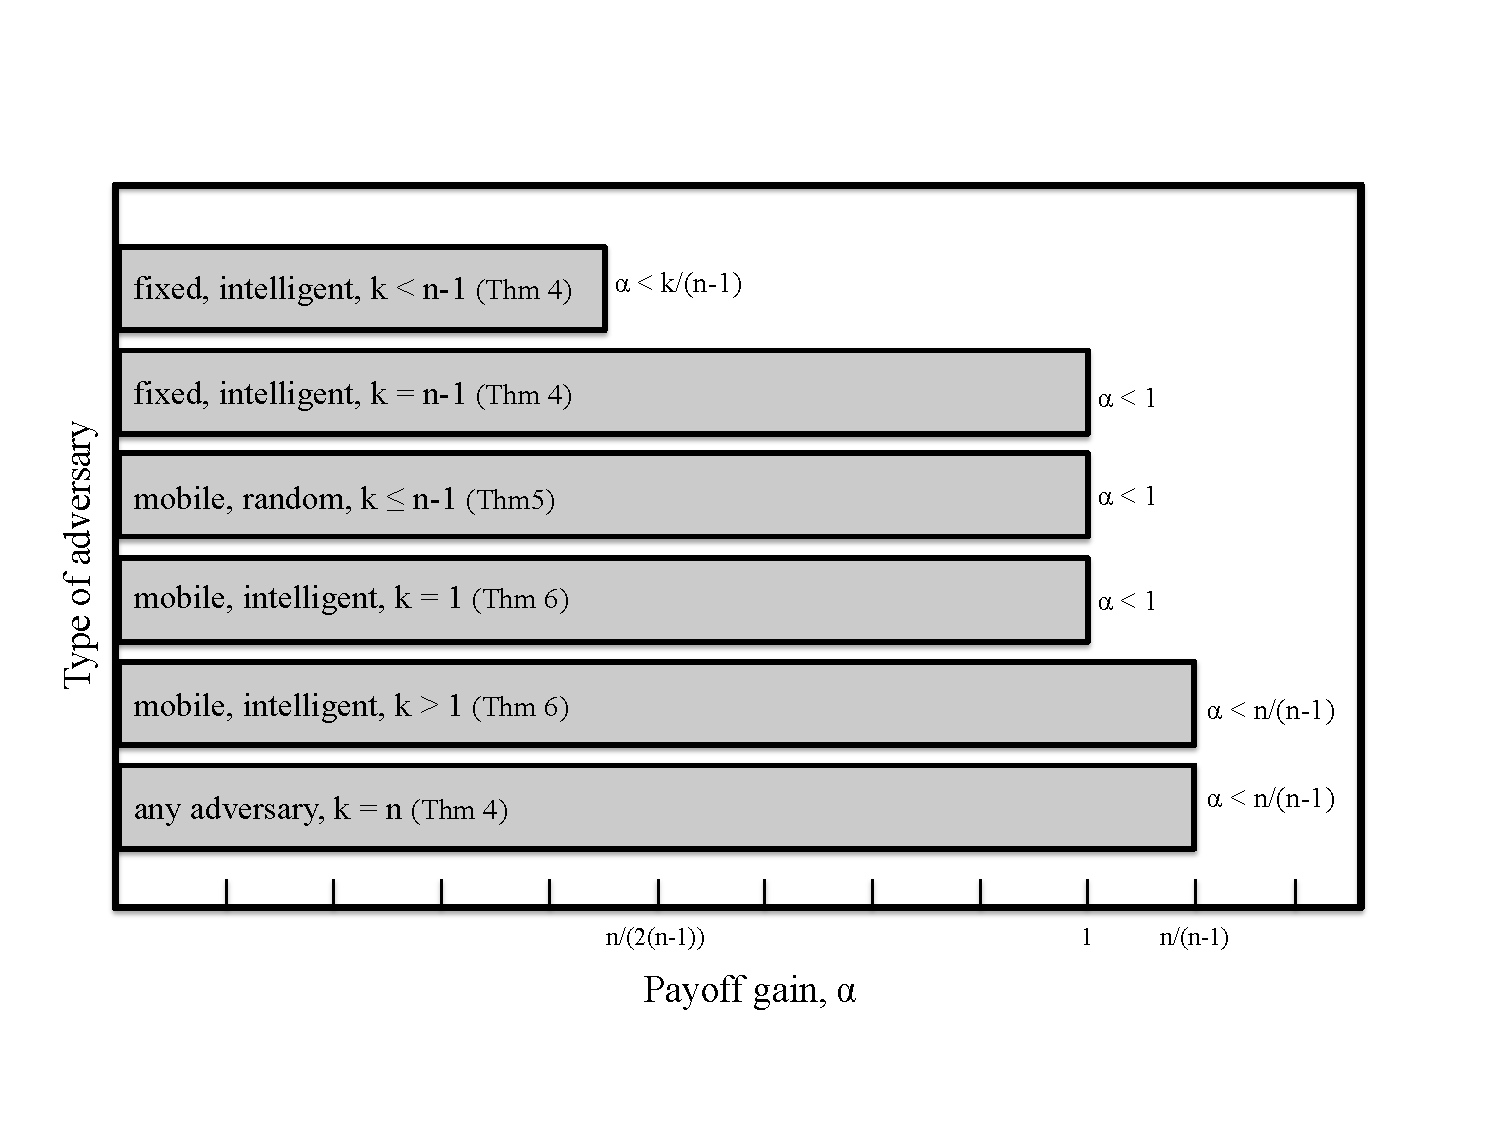
\includegraphics[width=.4\textwidth, clip, trim=10mm 10mm 20mm 30mm]{Presentation2}
  \caption{Values of $\alpha$ for which each type of adversary can stabilize joint action $\vec{y}$ in an $n$-agent line}\label{f:barGraph}
\end{figure}


